%% ---------------------------------------------------------------------------------------------------------
\section{Development results}\label{sec:dev}

\paragraph{Question} On development scenes, does V2 rescue failures without harming successes, and does its memory matter?

\begin{table}[!htbp]
\centering\footnotesize
\caption{Development stage (C1, seeds 51100--51299): successes of 200 scenes, rescues and harms against C0, and number of scenes in which the arm moved. The trigger fired in 195 (seed 1) and 191 (seed 2) scenes. For the oracle the column counts the scenes in which it entered its control loop (every trigger); it actually moved in 93 and 102.}\label{tab:dev}
\resizebox{\linewidth}{!}{\input{\tabdir T2_development_arms.tex}}
\end{table}

\begin{table}[!htbp]
\centering\footnotesize
\caption{Pre-registered development hypotheses (exact one-sided paired tests; Holm over the two hypotheses at $\alpha=0.05$, i.e.\ the smaller p-value is compared with 0.025 and the larger with 0.05; IU = intersection--union).}\label{tab:devtests}
\resizebox{\linewidth}{!}{\input{\tabdir T3_development_tests.tex}}
\end{table}

\paragraph{Evidence} Table~\ref{tab:dev} lists all nine arms. V2 raised success from 171 to 184 (14 rescues, 1 harm) for policy seed 1 and from 164 to 180 (16 rescues, 0 harms) for policy seed 2. The privileged oracle reached 185 and 184. Both pre-registered hypotheses were rejected (Table~\ref{tab:devtests}): V2 against C0 for policy seed 2 ($16$ vs $0$, $p=1.5\times10^{-5}$) and V2 against its single-frame variant for both policies (intersection--union $p=0.0078$).

\begin{figure}[!htbp]
\centering
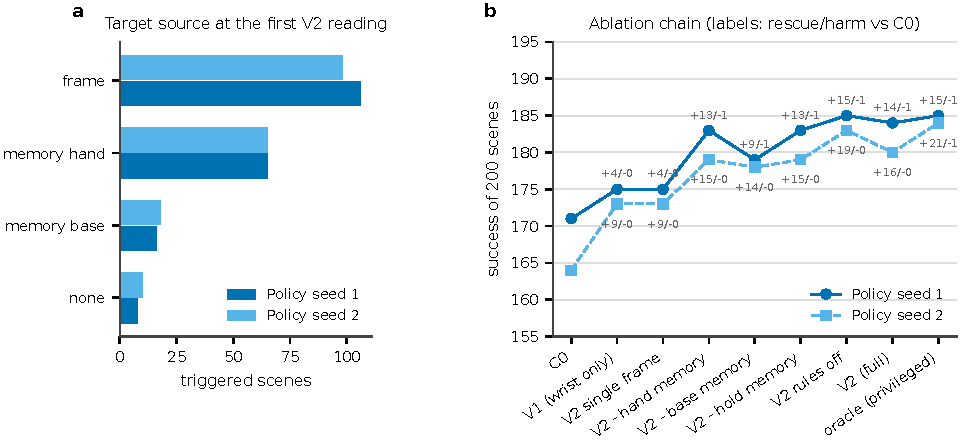
\includegraphics[width=\linewidth]{F4_memory_and_ablation.pdf}
\caption{Memory and ablation on the development scenes. (a) Source of the target estimate at the first V2 reading in triggered scenes: in about one third of them the target came from the wrist-camera memory, because the held cube hid it at the trigger. (b) Successes of all arms; labels give rescues/harms against C0. The single-frame variant behaves like the wrist-only V1, while removing one memory at a time loses less.}\label{fig:memory}
\end{figure}

\paragraph{Interpretation} Figure~\ref{fig:memory}a shows why memory matters: at the first reading the target position came from the current frame in 106 and 98 triggered scenes, from the hand memory in 65 and 65, and from the base memory in 16 and 18; in 8 and 10 there was no target estimate. Without confirmed memory (single frame) the controller acts in 25--30 scenes and rescues 4 and 9; with it, it acts in 39--41 scenes and rescues 14 and 16. Removing only the hand or the hold memory costs one rescue for seed 1 and one for seed 2, while removing the base memory costs five and two, which suggests that the memories partly substitute for each other.

\paragraph{Limits} The single-frame ablation sets the confirmation count to $m=1$, which also changes when a memory entry becomes usable; it is therefore not a pure removal of memory, and $H_{\mathrm{mem}}$ measures the combined effect (Section~\ref{sec:limits}). These are development results on scenes that informed the design; they do not certify a harm rate.

